% \chapter{Preface}
% other way 
\thispagestyle{empty}
\topskip0pt
\vspace*{4em}
\begin{center}
    {\bfseries\Huge Preface}
    \label{Preface}
    \pdfbookmark[0]{Preface}{}% 
\end{center}
\vspace*{5em}
This little book is especially concerned with those portions of
"advanced calculus" in which the subtlety of the concepts and
methods makes rigor difficult to attain at an elementary level.
The approach taken here uses elementary versions of modern
methods found in sophisticated mathematics. The formal
prerequisites include only a term of linear algebra, a nodding
acquaintance with the notation of set theory, and a respectable
first-year calculus course (one which at least mentions the
least upper bound (sup) and greatest lower bound (inf) of a
set of real numbers). Beyond this a certain (perhaps latent)
rapport with abstract mathematics will be found almost
essential.

The first half of the book covers that simple part of advanced 
calculus which generalizes elementary calculus to higher dimensions.
Chapter 1 contains preliminaries, and Chapters 2 and 3 treat 
differentiation and integration.The remainder of the book is devoted 
to the study of curves, surfaces, and higher-dimensional analogues.
Here the modern and classical treatments pursue quite different routes; 
there are, of course, many points of contact, and a significant encounter

The remainder of the book is devoted to the study of curves,
surfaces, and higher-dimensional analogues. Here the modern and classical 
treatments pursue quite different routes; there are, of course, 
many points of contact, and a significant encounter occurs 
in the last section. The very classical equation reproduced 
on the cover appears also as the last theorem of the
book. This theorem (Stokes' Theorem) has had a curious
history and has undergone a striking metamorphosis.

The first statement of the Theorem appears as a postscript
to a letter, dated July 2, 1850, from Sir William Thomson
(Lord Kelvin) to Stokes. It appeared publicly as question 8
on the Smith's Prize Examination for 1854.
This competitive examination, which was taken annually by the best 
mathematics students at Cambridge University, was set from 1849 to
1882 by Professor Stokes; by the time of his death the result
was known universally as Stokes' Theorem. At least three
proofs were given by his contemporaries: Thomson published
one, another appeared in Thomson and Tait's Treatise on
Natural Philosophy, and Maxwell provided another in Electricity 
and Magnetism \cite{maxwell1954electricity}. Since this time the name of
Stokes has been applied to much more general results, which
have figured so prominently in the development of certain
parts of mathematics that Stokes' Theorem may be con-
sidered a case study in the value of generalization.

In this book there are three forms of Stokes' Theorem.
The version known to Stokes appears in the last section, along
with its inseparable companions, Green's Theorem and the
Divergence Theorem.These three theorems, the classical
theorems of the subtitle, are derived quite easily from a
modern Stokes' Theorem which appears earlier in Chapter 5.
What the classical theorems state for curves and surfaces, this
theorem states for the higher-dimensional analogues (manifolds) 
which are studied thoroughly in the first part of Chapter
5.This study of manifolds, which could be justified solely on
the basis of their importance in modern mathematics, actually
involves no more effort than a careful study of curves and 
surfaces alone would require.

The reader probably suspects that the modern Stokes'
Theorem is at least as difficult as the classical theorems
derived from it.On the contrary, it is a very simple consequence of 
yet another version of Stokes' Theorem; this very
abstract version is the final and main result of Chapter 4.
It is entirely reasonable to suppose that the difficulties so far
avoided must be hidden here. Yet the proof of this theorem is, 
in the mathematician's sense, an utter triviality--a 
straightforward computation.On the other hand, even the statement
of this triviality cannot be understood without a horde of
difficult definitions from Chapter 4.There are good reasons
why the theorems should all be easy and the definitions hard.
As the evolution of Stokes' Theorem revealed, a single simple
principle, can masquerade as several difficult results; the proofs
of many theorems involve merely stripping away the disguise.
The definitions, on the other hand, serve a twofold purpose:
they are rigorous replacements for vague notions, and
machinery for elegant proofs.The first two sections of
Chapter 4 define precisely, and prove the rules for manipulating, 
what are classically described as "expressions of the form"
$P \dd x + Q\dd y + R\dd z$ or $P \dd x\dd y + Q\dd y\dd z + R\dd z\dd x$.
Chains,defined in the third section, and partitions of unity (already
introduced in Chapter 3) free our proofs from the necessity of
chopping manifolds up into small pieces; they reduce questions
about manifolds, where everything seems hard, to questions
about Euclidean space, where everything is easy.

Concentrating the depth of a subject in the definitions is
undeniably economical, but it is bound to produce some
difficulties for the student.I hope the reader will be encouraged to 
learn Chapter 4 thoroughly by the assurance that the
results will justify the effort: the classical theorems of the last
section represent only a few, and by no means the most 
important, applications of Chapter 4; many others appear as
problems, and further developments will be found by exploring
the bibliography.

The problems and the bibliography both deserve a few words. 
Problems appear after every section and are 
numbered (like the theorems) within chapters.I have starred
those problems whose results are used in the text, but this
precaution should be unnecessary-the problems are the most
important part of the book, and the reader should at least
attempt them all. It was necessary to make the bibliography
either very incomplete or unwieldy, since half the major 
branches of mathematics could legitimately be recommended
as reasonable continuations of the material in the book.
I have tried to make it incomplete but tempting.

Many criticisms and suggestions were offered during the
writing of this book.I am particularly grateful to Richard
Palais, Hugo Rossi, Robert Seeley, and Charles Stenard for
their many helpful comments.

I have used this printing as an opportunity to correct many
misprints and minor errors pointed out to me by indulgent
readers. In addition, the material following Theorem 3-11
has been completely revised and corrected. Other important
changes, which could not be incorporated in the text without
excessive alteration, are listed in the Addenda at the end of the
book.

\vspace*{1em}
\hspace*{\fill}\textbf{\itshape Michael Spivak}\par 
\noindent {\itshape Waltham, Massachusetts}\par 
\noindent {\itshape March 1968}\par 

\newpage
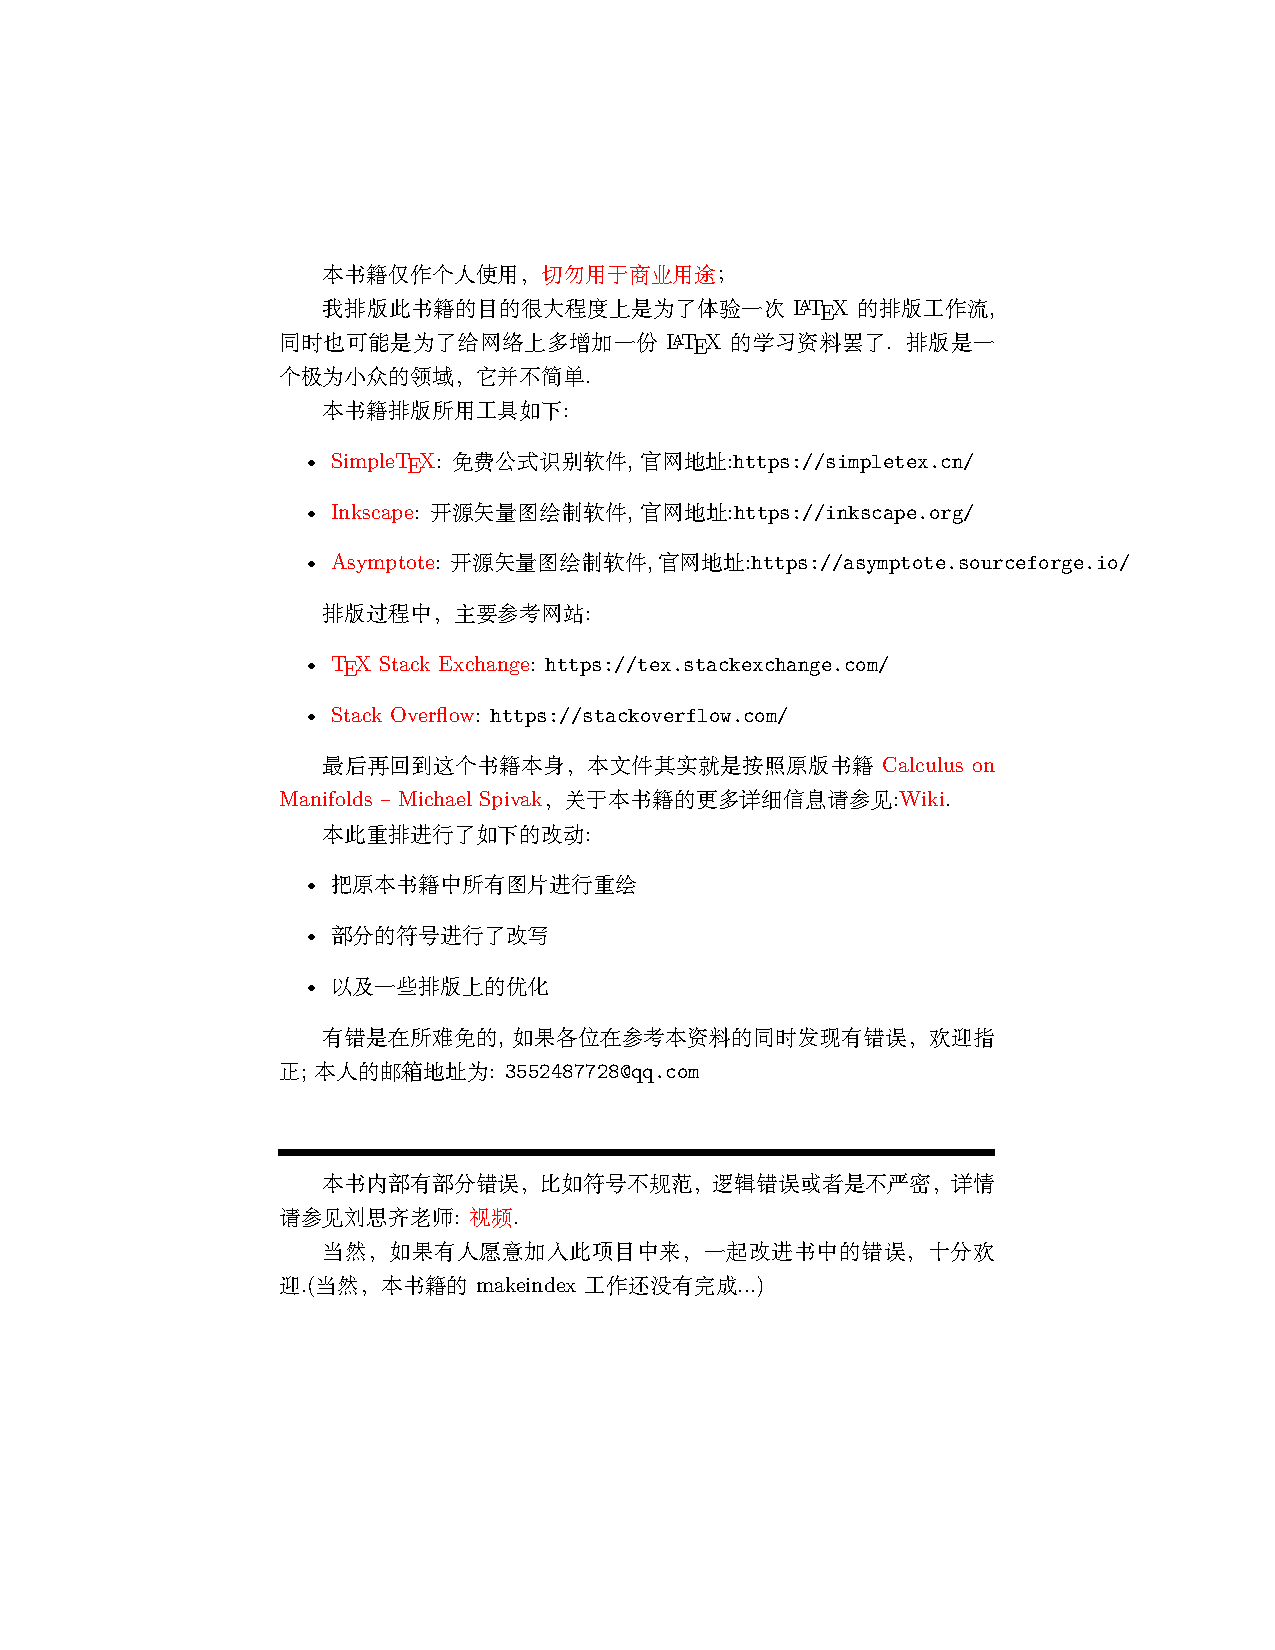
\includepdf{./chapter/NoteThat.pdf}
